\section{Выигрыш игрока Студент}

Теперь на квадрате $(\mu, \lambda) \in [0, 1]^2$ мы рассмотрели все точки
и для каждой нашли оптимальные пары $p^*(\mu, \lambda)$
и $q^*(\mu, \lambda)$ и соответсвующие значения функции 
$M(p^*(\mu, \lambda),q^*(\mu, \lambda),\mu)$. Далее на квадрате
$[0, 1]^{2}$ изобразим все точки, которые принимает вектор $(\mu M(p^*,q^*,\mu), (1-\mu) M(p^*,q^*,\mu))$ при
$(\mu, \lambda)\in[0, 1]^{2}$

\begin{center}
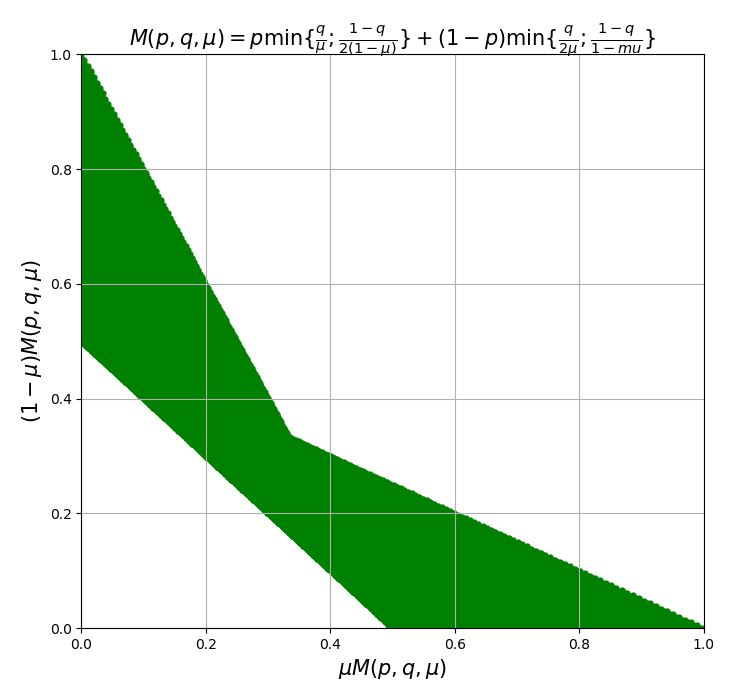
\includegraphics[scale=0.6]{part_2/graf_4}
\end{center}

Поясним график: \\
нижняя огибающая в координатах $X,Y$: $y=\dfrac{1}{2}-x$, \\
верхняя огибающая в координатах $X,Y$: 
$y=
\begin{cases}
	1 - 2x, & x \in [0, \dfrac{1}{3}) \\
	\dfrac{1 - x}{2}, & x \in [\dfrac{1}{3}, 1]
\end{cases}.
$

И найдём множества значений функции 

$$
	\overline G(p, q, \mu)=
	p \min \{
		\dfrac{q}{\mu};
		\dfrac{1-q}{2(1-\mu)}
	\} + (1 - p) \min \{
		\dfrac{q}{2\mu};
		\dfrac{1 - q}{1 - \mu}
	\},
$$

В этих областях
Далее рассмотрим игру с точки зрения игрока С. 
найдём значение свёртки для игрока С в этих точка:

, тогда

$
	\overline G(1, 0, 0) = \dfrac{1}{2}
$

$
	\overline G([0, 1], 0, 0) = [0.5, 1]
$

$	
	\overline G([0, 1], 1, 1) = [0.5, 1]
$

$
	\overline G(1, \dfrac{\mu}{2 - \mu}, \mu)=
	\min \big\{
		\dfrac{\mu}{2 - \mu}; 
		\dfrac{1 - \dfrac{\mu}{2 - \mu}}{2(1 - \mu)}
	\big\}
	=\dfrac{1}{2 - \mu}
$

$
	\overline G(1,\dfrac{\mu}{2-\mu},\mu)=\dfrac{1}{2-\mu}
$

$
	\overline G(p,\dfrac{2\mu}{1+\mu},\mu) =
	p\dfrac{1}{2(1 + \mu)} + (1 - p)\dfrac{1}{1 + \mu}=
	\dfrac{2 - p}{2(1 + \mu)} \geqslant
	\dfrac{2 - (1 - \mu)}{2(1 + \mu)} =
	\dfrac{1 + \mu}{2(1 + \mu)} =
	\dfrac{1}{2}
$

$
	\overline G(p, \dfrac{2\mu}{1 + \mu}, \mu) \leqslant 
	\dfrac{1}{1 + \mu} \Rightarrow
	\overline G (p, \dfrac{2\mu}{1 + \mu}, \mu) = 
	[0.5, 	\dfrac{1}{1 + \mu}]
$

$
	\overline G(0, \dfrac{2\mu}{1 + \mu}, \mu) = 
	\dfrac{1}{1 + \mu}
$

$
	\overline G(1, \dfrac{\mu}{2 - \mu}, \mu) = 
	\dfrac{1}{2 - \mu}
$

$
	\overline G(0, \dfrac{2\mu}{1 + \mu}, \mu) = 
	\dfrac{1}{1 + \mu}
$

$
	\overline G(p, \dfrac{\mu}{2 - \mu}, \mu) =
	p\dfrac{1}{2 - \mu} + (1 - p)\dfrac{1}{2(2 - \mu)} =
	\dfrac{1 + p}{2(2 - \mu)} \geqslant 
	\dfrac{2 - \mu}{2(2 - \mu)} =
	\dfrac{1}{2}
$

$
	\overline G(p, \dfrac{\mu}{2 - \mu}, \mu) \leqslant
 	\dfrac{1}{2 - \mu} \Rightarrow 
 	\overline G(p, \dfrac{\mu}{2 - \mu}, \mu) =
 	[0.5, \dfrac{1}{2 - \mu}]
$

$
	\overline G(0, \dfrac{2\mu}{1 + \mu}, \mu)=
	\min \big\{
		\dfrac{1}{\mu}\dfrac{2\mu}{1 + \mu}; 
		\dfrac{1 - \dfrac{2\mu}{1 + \mu}}{1 - \mu}
	\big\} =
	\dfrac{1}{1 + \mu}
$

$
	\overline G(0, 1, 1) = \dfrac{1}{2}
$